\PassOptionsToPackage{unicode=true}{hyperref} % options for packages loaded elsewhere
\PassOptionsToPackage{hyphens}{url}
%
\documentclass[]{article}
\usepackage{lmodern}
\usepackage{amssymb,amsmath}
\usepackage{ifxetex,ifluatex}
\usepackage{fixltx2e} % provides \textsubscript
\ifnum 0\ifxetex 1\fi\ifluatex 1\fi=0 % if pdftex
  \usepackage[T1]{fontenc}
  \usepackage[utf8]{inputenc}
  \usepackage{textcomp} % provides euro and other symbols
\else % if luatex or xelatex
  \usepackage{unicode-math}
  \defaultfontfeatures{Ligatures=TeX,Scale=MatchLowercase}
\fi
% use upquote if available, for straight quotes in verbatim environments
\IfFileExists{upquote.sty}{\usepackage{upquote}}{}
% use microtype if available
\IfFileExists{microtype.sty}{%
\usepackage[]{microtype}
\UseMicrotypeSet[protrusion]{basicmath} % disable protrusion for tt fonts
}{}
\IfFileExists{parskip.sty}{%
\usepackage{parskip}
}{% else
\setlength{\parindent}{0pt}
\setlength{\parskip}{6pt plus 2pt minus 1pt}
}
\usepackage{hyperref}
\hypersetup{
            pdftitle={Week 1 exercises},
            pdfauthor={Daniel Alonso},
            pdfborder={0 0 0},
            breaklinks=true}
\urlstyle{same}  % don't use monospace font for urls
\usepackage[margin=1in]{geometry}
\usepackage{color}
\usepackage{fancyvrb}
\newcommand{\VerbBar}{|}
\newcommand{\VERB}{\Verb[commandchars=\\\{\}]}
\DefineVerbatimEnvironment{Highlighting}{Verbatim}{commandchars=\\\{\}}
% Add ',fontsize=\small' for more characters per line
\usepackage{framed}
\definecolor{shadecolor}{RGB}{248,248,248}
\newenvironment{Shaded}{\begin{snugshade}}{\end{snugshade}}
\newcommand{\AlertTok}[1]{\textcolor[rgb]{0.94,0.16,0.16}{#1}}
\newcommand{\AnnotationTok}[1]{\textcolor[rgb]{0.56,0.35,0.01}{\textbf{\textit{#1}}}}
\newcommand{\AttributeTok}[1]{\textcolor[rgb]{0.77,0.63,0.00}{#1}}
\newcommand{\BaseNTok}[1]{\textcolor[rgb]{0.00,0.00,0.81}{#1}}
\newcommand{\BuiltInTok}[1]{#1}
\newcommand{\CharTok}[1]{\textcolor[rgb]{0.31,0.60,0.02}{#1}}
\newcommand{\CommentTok}[1]{\textcolor[rgb]{0.56,0.35,0.01}{\textit{#1}}}
\newcommand{\CommentVarTok}[1]{\textcolor[rgb]{0.56,0.35,0.01}{\textbf{\textit{#1}}}}
\newcommand{\ConstantTok}[1]{\textcolor[rgb]{0.00,0.00,0.00}{#1}}
\newcommand{\ControlFlowTok}[1]{\textcolor[rgb]{0.13,0.29,0.53}{\textbf{#1}}}
\newcommand{\DataTypeTok}[1]{\textcolor[rgb]{0.13,0.29,0.53}{#1}}
\newcommand{\DecValTok}[1]{\textcolor[rgb]{0.00,0.00,0.81}{#1}}
\newcommand{\DocumentationTok}[1]{\textcolor[rgb]{0.56,0.35,0.01}{\textbf{\textit{#1}}}}
\newcommand{\ErrorTok}[1]{\textcolor[rgb]{0.64,0.00,0.00}{\textbf{#1}}}
\newcommand{\ExtensionTok}[1]{#1}
\newcommand{\FloatTok}[1]{\textcolor[rgb]{0.00,0.00,0.81}{#1}}
\newcommand{\FunctionTok}[1]{\textcolor[rgb]{0.00,0.00,0.00}{#1}}
\newcommand{\ImportTok}[1]{#1}
\newcommand{\InformationTok}[1]{\textcolor[rgb]{0.56,0.35,0.01}{\textbf{\textit{#1}}}}
\newcommand{\KeywordTok}[1]{\textcolor[rgb]{0.13,0.29,0.53}{\textbf{#1}}}
\newcommand{\NormalTok}[1]{#1}
\newcommand{\OperatorTok}[1]{\textcolor[rgb]{0.81,0.36,0.00}{\textbf{#1}}}
\newcommand{\OtherTok}[1]{\textcolor[rgb]{0.56,0.35,0.01}{#1}}
\newcommand{\PreprocessorTok}[1]{\textcolor[rgb]{0.56,0.35,0.01}{\textit{#1}}}
\newcommand{\RegionMarkerTok}[1]{#1}
\newcommand{\SpecialCharTok}[1]{\textcolor[rgb]{0.00,0.00,0.00}{#1}}
\newcommand{\SpecialStringTok}[1]{\textcolor[rgb]{0.31,0.60,0.02}{#1}}
\newcommand{\StringTok}[1]{\textcolor[rgb]{0.31,0.60,0.02}{#1}}
\newcommand{\VariableTok}[1]{\textcolor[rgb]{0.00,0.00,0.00}{#1}}
\newcommand{\VerbatimStringTok}[1]{\textcolor[rgb]{0.31,0.60,0.02}{#1}}
\newcommand{\WarningTok}[1]{\textcolor[rgb]{0.56,0.35,0.01}{\textbf{\textit{#1}}}}
\usepackage{graphicx,grffile}
\makeatletter
\def\maxwidth{\ifdim\Gin@nat@width>\linewidth\linewidth\else\Gin@nat@width\fi}
\def\maxheight{\ifdim\Gin@nat@height>\textheight\textheight\else\Gin@nat@height\fi}
\makeatother
% Scale images if necessary, so that they will not overflow the page
% margins by default, and it is still possible to overwrite the defaults
% using explicit options in \includegraphics[width, height, ...]{}
\setkeys{Gin}{width=\maxwidth,height=\maxheight,keepaspectratio}
\setlength{\emergencystretch}{3em}  % prevent overfull lines
\providecommand{\tightlist}{%
  \setlength{\itemsep}{0pt}\setlength{\parskip}{0pt}}
\setcounter{secnumdepth}{0}
% Redefines (sub)paragraphs to behave more like sections
\ifx\paragraph\undefined\else
\let\oldparagraph\paragraph
\renewcommand{\paragraph}[1]{\oldparagraph{#1}\mbox{}}
\fi
\ifx\subparagraph\undefined\else
\let\oldsubparagraph\subparagraph
\renewcommand{\subparagraph}[1]{\oldsubparagraph{#1}\mbox{}}
\fi

% set default figure placement to htbp
\makeatletter
\def\fps@figure{htbp}
\makeatother


\title{Week 1 exercises}
\author{Daniel Alonso}
\date{November 18th, 2020}

\begin{document}
\maketitle

Importing libraries

\begin{Shaded}
\begin{Highlighting}[]
\KeywordTok{library}\NormalTok{(ggplot2)}
\KeywordTok{library}\NormalTok{(foreach)}
\KeywordTok{library}\NormalTok{(dplyr)}
\end{Highlighting}
\end{Shaded}

\hypertarget{exercise-1}{%
\subsection{Exercise 1}\label{exercise-1}}

Simulating 100 trajectories of length \(n = 1000\) for \(X\) and \(Y\).

\begin{Shaded}
\begin{Highlighting}[]
\NormalTok{Traj_X <-}\StringTok{ }\KeywordTok{data.frame}\NormalTok{()}
\NormalTok{Traj_Y <-}\StringTok{ }\KeywordTok{data.frame}\NormalTok{()}
\ControlFlowTok{for}\NormalTok{ (k }\ControlFlowTok{in} \DecValTok{1}\OperatorTok{:}\DecValTok{100}\NormalTok{) \{}
\NormalTok{    X <-}\StringTok{ }\KeywordTok{data.frame}\NormalTok{(}\DataTypeTok{x=}\DecValTok{1}\OperatorTok{:}\DecValTok{1000}\NormalTok{,}\DataTypeTok{val=}\KeywordTok{rep}\NormalTok{(}\DecValTok{0}\NormalTok{,}\DecValTok{1000}\NormalTok{),}\DataTypeTok{run=}\KeywordTok{rep}\NormalTok{(k,}\DecValTok{1000}\NormalTok{))}
\NormalTok{    Y <-}\StringTok{ }\KeywordTok{data.frame}\NormalTok{(}\DataTypeTok{x=}\DecValTok{1}\OperatorTok{:}\DecValTok{1000}\NormalTok{,}\DataTypeTok{val=}\KeywordTok{rep}\NormalTok{(}\DecValTok{0}\NormalTok{,}\DecValTok{1000}\NormalTok{),}\DataTypeTok{run=}\KeywordTok{rep}\NormalTok{(k,}\DecValTok{1000}\NormalTok{))}
\NormalTok{    X_r <-}\StringTok{ }\KeywordTok{rep}\NormalTok{(}\DecValTok{0}\NormalTok{,}\DecValTok{1000}\NormalTok{)}
\NormalTok{    Y_r <-}\StringTok{ }\KeywordTok{rep}\NormalTok{(}\DecValTok{0}\NormalTok{,}\DecValTok{1000}\NormalTok{)}
    \ControlFlowTok{for}\NormalTok{ (i }\ControlFlowTok{in} \DecValTok{1}\OperatorTok{:}\DecValTok{1000}\NormalTok{) \{}
        \ControlFlowTok{if}\NormalTok{ (i }\OperatorTok{>}\StringTok{ }\DecValTok{1}\NormalTok{) \{}
\NormalTok{            X_r[i] <-}\StringTok{ }\FloatTok{0.5}\OperatorTok{*}\NormalTok{X_r[i}\DecValTok{-1}\NormalTok{]}\OperatorTok{+}\KeywordTok{rnorm}\NormalTok{(}\DecValTok{1}\NormalTok{)}
\NormalTok{            Y_r[i] <-}\StringTok{ }\DecValTok{2}\OperatorTok{*}\NormalTok{Y_r[i}\DecValTok{-1}\NormalTok{]}\OperatorTok{+}\KeywordTok{rnorm}\NormalTok{(}\DecValTok{1}\NormalTok{)}
\NormalTok{        \}}
\NormalTok{    \}}
\NormalTok{    X}\OperatorTok{$}\NormalTok{val <-}\StringTok{ }\NormalTok{X_r}
\NormalTok{    Y}\OperatorTok{$}\NormalTok{val <-}\StringTok{ }\NormalTok{Y_r}
\NormalTok{    Traj_X <-}\StringTok{ }\KeywordTok{rbind}\NormalTok{(Traj_X, X)}
\NormalTok{    Traj_Y <-}\StringTok{ }\KeywordTok{rbind}\NormalTok{(Traj_Y, Y)}
\NormalTok{\}}
\end{Highlighting}
\end{Shaded}

\newpage

\hypertarget{a---plotting-simulated-trajectories}{%
\subsubsection{a - Plotting simulated
trajectories}\label{a---plotting-simulated-trajectories}}

\hypertarget{trajectories-x}{%
\paragraph{Trajectories X}\label{trajectories-x}}

\begin{Shaded}
\begin{Highlighting}[]
\KeywordTok{ggplot}\NormalTok{(}\DataTypeTok{data =}\NormalTok{ Traj_X, }\KeywordTok{aes}\NormalTok{(}\DataTypeTok{x=}\NormalTok{x, }\DataTypeTok{y=}\NormalTok{val)) }\OperatorTok{+}\StringTok{ }
\StringTok{    }\KeywordTok{geom_line}\NormalTok{(}\KeywordTok{aes}\NormalTok{(}\DataTypeTok{colour=}\NormalTok{run), }\DataTypeTok{show.legend=}\OtherTok{FALSE}\NormalTok{)}
\end{Highlighting}
\end{Shaded}

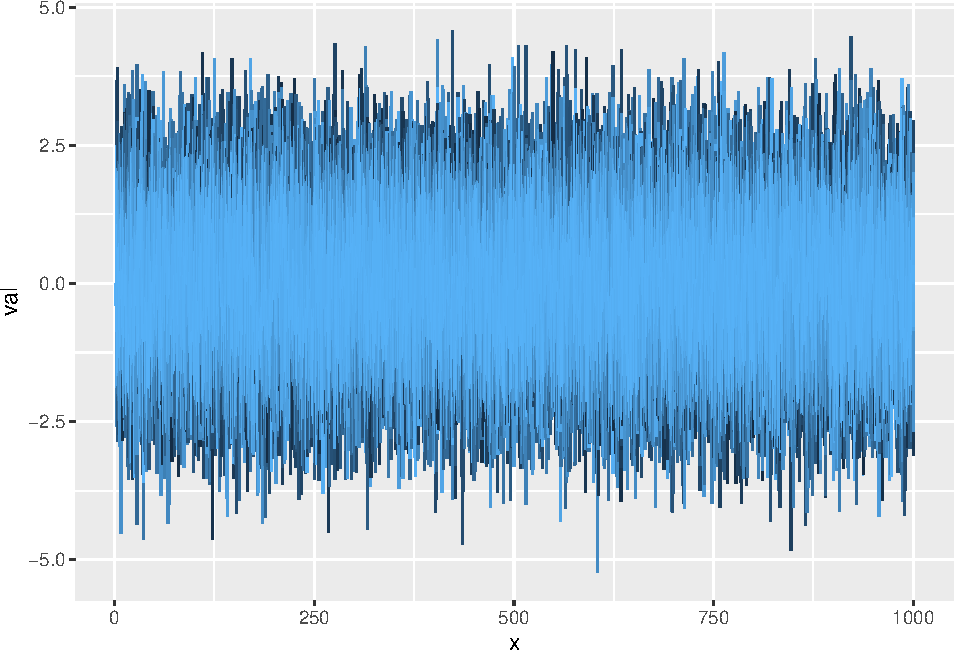
\includegraphics{ex1_report_files/figure-latex/unnamed-chunk-3-1.pdf}

\hypertarget{trajectories-y}{%
\paragraph{Trajectories Y}\label{trajectories-y}}

The values of Y are too large for ggplot to show.

\hypertarget{b---use-the-simulated-trajectories-to-estimate-the-mean-and-the-covariance-functions}{%
\subsubsection{b - Use the simulated trajectories to estimate the mean
and the covariance
functions}\label{b---use-the-simulated-trajectories-to-estimate-the-mean-and-the-covariance-functions}}

\begin{Shaded}
\begin{Highlighting}[]
\NormalTok{mean_X =}\StringTok{ }\KeywordTok{rep}\NormalTok{(}\DecValTok{0}\NormalTok{,}\DecValTok{100}\NormalTok{)}
\NormalTok{mean_Y =}\StringTok{ }\KeywordTok{rep}\NormalTok{(}\DecValTok{0}\NormalTok{,}\DecValTok{100}\NormalTok{)}
\ControlFlowTok{for}\NormalTok{ (i }\ControlFlowTok{in} \DecValTok{1}\OperatorTok{:}\DecValTok{100}\NormalTok{) \{}
\NormalTok{    x =}\StringTok{ }\NormalTok{Traj_X }\OperatorTok\StringTok{ }\KeywordTok{filter}\NormalTok{(run }\OperatorTok{==}\StringTok{ }\NormalTok{i) }\OperatorTok\StringTok{ }\KeywordTok{select}\NormalTok{(val)}
\NormalTok{    y =}\StringTok{ }\NormalTok{Traj_Y }\OperatorTok\StringTok{ }\KeywordTok{filter}\NormalTok{(run }\OperatorTok{==}\StringTok{ }\NormalTok{i) }\OperatorTok\StringTok{ }\KeywordTok{select}\NormalTok{(val)}
\NormalTok{    mean_X[i] =}\StringTok{ }\KeywordTok{mean}\NormalTok{(x}\OperatorTok{$}\NormalTok{val)}
\NormalTok{    mean_Y[i] =}\StringTok{ }\KeywordTok{mean}\NormalTok{(y}\OperatorTok{$}\NormalTok{val)}
\NormalTok{\}}
\end{Highlighting}
\end{Shaded}

The mean of all trajectories of X is the following:

\begin{Shaded}
\begin{Highlighting}[]
\KeywordTok{mean}\NormalTok{(mean_X)}
\end{Highlighting}
\end{Shaded}

\begin{verbatim}
## [1] -0.002558796
\end{verbatim}

The mean of all trajectories of Y is the following:

\begin{Shaded}
\begin{Highlighting}[]
\KeywordTok{mean}\NormalTok{(mean_Y)}
\end{Highlighting}
\end{Shaded}

\begin{verbatim}
## [1] -5.629677e+296
\end{verbatim}

The mean of the covariances of all combinations of trajectories is the
following:

\begin{Shaded}
\begin{Highlighting}[]
\NormalTok{covs =}\StringTok{ }\KeywordTok{rep}\NormalTok{(}\DecValTok{0}\NormalTok{,}\DecValTok{100}\OperatorTok{*}\DecValTok{100}\NormalTok{)}
\NormalTok{cnt =}\StringTok{ }\DecValTok{0}
\ControlFlowTok{for}\NormalTok{ (i }\ControlFlowTok{in} \DecValTok{1}\OperatorTok{:}\DecValTok{100}\NormalTok{) \{}
    \ControlFlowTok{for}\NormalTok{ (j }\ControlFlowTok{in} \DecValTok{1}\OperatorTok{:}\DecValTok{100}\NormalTok{) \{}
\NormalTok{        x =}\StringTok{ }\NormalTok{Traj_X }\OperatorTok\StringTok{ }\KeywordTok{filter}\NormalTok{(run }\OperatorTok{==}\StringTok{ }\NormalTok{i) }\OperatorTok\StringTok{ }\KeywordTok{select}\NormalTok{(val)}
\NormalTok{        y =}\StringTok{ }\NormalTok{Traj_Y }\OperatorTok\StringTok{ }\KeywordTok{filter}\NormalTok{(run }\OperatorTok{==}\StringTok{ }\NormalTok{j) }\OperatorTok\StringTok{ }\KeywordTok{select}\NormalTok{(val)}
\NormalTok{        cnt =}\StringTok{ }\NormalTok{cnt }\OperatorTok{+}\StringTok{ }\DecValTok{1}
\NormalTok{        covs[cnt] =}\StringTok{ }\KeywordTok{cov}\NormalTok{(x,y)}
\NormalTok{    \}}
\NormalTok{\}}
\KeywordTok{mean}\NormalTok{(covs)}
\end{Highlighting}
\end{Shaded}

\begin{verbatim}
## [1] -4.211591e+295
\end{verbatim}

\end{document}
